\section{Architecture Structure}\label{sec:4}

\subsection{Candidate Architecture Styles}\label{sec:4.1}

Six architecture families are evaluated as concrete VinaBeef variants,
using the course trade-off framework and supplemental style
descriptions. The comparison also includes V2E, a modular
central monolith with the same farm edge as V4, so placement benefits
are not mistaken for benefits unique to service-based architecture. D-01
Reliability/Durability, D-02 Performance and D-03 Security/Auditability
are primary; Availability is secondary.


\begin{itemize}
  \item \textbf{V1 Layered monolith:} one central deployable unit with presentation, business and persistence layers. Readers send every read across the WAN to the central site. A single ACID database makes it easy to commit a business effect and its evidence atomically (D-01, D-03). However, every read' s deadline then depends on WAN latency (D-02), and gate processing stops during an outage.
  \item \textbf{V2 Modular monolith:} the same deployment as V1, split internally into domain modules (Movement, Health, Registry, Alerting). Module boundaries are clearer than in V1, but it has the same timing and continuity limits.
  \item \textbf{V3 Microkernel:} a core system with plug-ins for reader protocols, report exporters and API adapters. This suits adapter variation (NFR-08) but does not structure the whole system, and plug-ins widen the trust boundary.
  \item \textbf{V4 Service-based with farm edge:} a few coarse-grained domain services, each owning its own schema, plus an edge gateway at each farm that completes gate processing locally.
  \item \textbf{V5 Event-driven (broker topology):} every processing step reacts to events through a central broker. This buffers bursts and decouples producers from consumers. However, each hop adds latency, and a broker acknowledgement does not prove that the business outcome is complete. Authorization and audit context are also harder to trace across asynchronous chains.
  \item V2E Modular monolith with farm edge: the same qualified local core, commit boundary and offline subset as V4, but one modular central deployable application. Local deadline and outage support are comparable; central deployment and process-resource isolation differ.
  \item V6 Microservices with the same farm edge: each farm runs the same local core, atomic commit boundary and offline subset as V4. Only the central backend is decomposed into finer-grained services with separately owned databases. WAN and central broker hops are outside the local gate deadline. Cross-owner workflows may need durable coordination; the added authorization, evidence and deployment boundaries require qualification.
\end{itemize}


\subsection{Comparison}\label{sec:4.2}

Each variant is rated from 1 (poor fit) to 5 (excellent fit) for this
project. The three drivers have weight 3, Availability has weight 2, and
Simplicity/Cost and Evolvability have weight 1 each; the maximum is 65.
Ratings are the group's assessments of the stated design and control effort,
not measured guarantees or inherent limits of a style. V4, V2E and V6
share the same local gate core, so their local Performance and
normal-operation Reliability/Durability ratings are equal. V6 scores
47/65; its additional central policy/evidence boundaries and deployment
cost drive the remaining differences.

{\footnotesize
\begin{longtable}[]{|>{\raggedright\arraybackslash}p{\dimexpr 0.1678\linewidth-2\tabcolsep\relax}|>{\raggedright\arraybackslash}p{\dimexpr 0.1162\linewidth-2\tabcolsep\relax}|>{\raggedright\arraybackslash}p{\dimexpr 0.1340\linewidth-2\tabcolsep\relax}|>{\raggedright\arraybackslash}p{\dimexpr 0.1243\linewidth-2\tabcolsep\relax}|>{\raggedright\arraybackslash}p{\dimexpr 0.1211\linewidth-2\tabcolsep\relax}|>{\raggedright\arraybackslash}p{\dimexpr 0.1114\linewidth-2\tabcolsep\relax}|>{\raggedright\arraybackslash}p{\dimexpr 0.1226\linewidth-2\tabcolsep\relax}|>{\raggedright\arraybackslash}p{\dimexpr 0.0727\linewidth-2\tabcolsep\relax}|}
\hline
\textbf{Variant} & \textbf{D-01 Reliability / Durability (\(\times\)3)} & \textbf{D-02 Performance (\(\times\)3)} & \textbf{D-03 Security / Auditability (\(\times\)3)} & \textbf{Avail\-abil\-ity (\(\times\)2)} & \textbf{Sim\-plic\-ity / Cost (\(\times\)1)} & \textbf{Evolv\-abil\-ity (\(\times\)1)} & \textbf{Total} \\ \hline
\endhead
\textbf{V1 Layered monolith} & 3 & 2 & 4 & 1 & 5 & 1 & 35 \\ \hline
\textbf{V2 Modular monolith} & 3 & 2 & 4 & 1 & 4 & 2 & 35 \\ \hline
\textbf{V3 Microkernel} & 3 & 2 & 3 & 1 & 4 & 3 & 33 \\ \hline
\textbf{V4 Service-based + farm edge} & \textbf{4} & \textbf{4} &
\textbf{4} & \textbf{4} & \textbf{3} & \textbf{3} & \textbf{50} \\ \hline
\textbf{V5 Event-driven} & 4 & 3 & 2 & 3 & 2 & 4 & 39 \\ \hline
V6 Microservices + same farm edge & 4 & 4 & 3 & 4 & 1 & 5 & 47 \\ \hline
V2E Modular monolith + same farm edge & 4 & 4 & 4 & 4 & 4 & 2 & 50 \\ \hline
\end{longtable}
}

\textbf{Rationale per driver}


\begin{itemize}
  \item \textbf{D-01 Reliability/Durability:}
  \begin{itemize}
    \item The explicitly central-only variants V1--V3 score 3 under this comparison. A single database supports atomic commits, but source capture and WAN receipt still require qualified protection. This is not an inherent prohibition on adding an edge to a monolith.
    \item V4 commits each read at the edge together with its operation identity and evidence before acknowledging it. It then relays the read through an outbox to central.
    \item V5 has a durable broker and replay, but scores only 4 because the broker acknowledgement must not be mistaken for business completion.
    \item V2E and V6 use the same farm-local commit contract as V4 and receive the same Reliability/Durability rating of 4. V6 must preserve receipts, source evidence and owned recovery for central workflows; separate databases do not inherently lose records. Cross-owner workflows require explicit coordination where atomicity cannot be kept within one owner.
  \end{itemize}
  \item \textbf{D-02 Performance:} the \(\leq\)2 second deadline applies to every read, so what matters is where processing completes and how many hops lie on the critical path, not average throughput.
  \begin{itemize}
    \item V4, V2E and the stated V6 all complete the same gate outcome on the farm LAN and receive Performance 4. Their central decomposition does not add a WAN or central broker hop to this local completion path.
    \item In V1--V3, every read depends on the WAN.
    \item The stated V5 broker topology puts central broker/network hops on the gate path. V6 does not: only its central backend is split into microservices. Resource contention and actual timing must still be measured in M2 for every variant.
  \end{itemize}
  \item \textbf{D-03 Security/Auditability:}
  \begin{itemize}
    \item V1, V2, V2E and V4 have few authorization boundaries and can commit source evidence in the same transaction as the business change.
    \item V5 carries authorization/evidence context across asynchronous chains. V6 receives Security/Auditability 3 because its finer central boundaries add policy propagation, evidence correlation and review effort. It can satisfy the same mandatory controls; this rating assesses project fit, not permission correctness or audit loss already observed in an implementation.
  \end{itemize}
  \item Availability (secondary): V4, V2E and the stated V6 have the same farm-local core, offline subset and Availability rating of 4. Central service granularity does not determine whether this gate subset survives WAN loss.
\end{itemize}


\subsection{Selected Style}\label{sec:4.3}

\textbf{Decision: V4 is selected. V4 and V2E both score 50/65, and V6
with the same farm edge scores 47/65; all three can implement the same
local gate contracts. V4 is chosen for explicit ownership and separate
process/deployment boundaries between movement, clinical work,
reporting/integration and identity/admin, with fewer central service
units than V6. V2E remains a credible alternative with simpler central
deployment. The shared central PostgreSQL server remains a common fault
domain, mitigated by the synchronous standby and backups in
\Cref{sec:4.5}.}


\begin{itemize}
  \item \textbf{D-01 Reliability/Durability:}
  \begin{itemize}
    \item The edge commits the movement, count effect, operation identity and source evidence in one local transaction before it acknowledges the read.
    \item A transactional outbox relays the committed facts to central at least once. Stable identities make replays idempotent.
  \end{itemize}
  \item \textbf{D-02 Performance:}
  \begin{itemize}
    \item The critical path from read to durable local outcome stays inside one farm, with no WAN, central broker or external API on it.
    \item Central synchronization, reporting and National API delivery run outside the deadline path.
    \item Resource isolation on the edge is still required. Local placement makes the deadline achievable but does not guarantee it.
  \end{itemize}
  \item \textbf{D-03 Security/Auditability:}
  \begin{itemize}
    \item A small number of coarse-grained services keeps authorization and evidence ownership clear. Each service authorizes against its own resources and commits its audit evidence in the same transaction as the change.
    \item The API gateway authenticates users and applies coarse checks. Services re-check permissions on the canonical resource, because gateway checks alone are insufficient.
  \end{itemize}
  \item \textbf{Role of event-driven:} events propagate facts that are already committed: edge to central, movement to head count and alerts, and health records to integration. This keeps the benefits of buffering and decoupling without putting broker hops on the deadline path.
  \item \textbf{Availability (secondary):} the same edge placement lets gate processing continue during a WAN outage.
  \item \textbf{Rejected -- central-only V1/V2:} their gate outcomes depend on the WAN. This does not reject modular monolith + edge (V2E), which remains a viable alternative; V4 is preferred for central domain ownership and isolation.
  \item \textbf{Rejected -- V5 pure event-driven:} broker hops on the critical path, and audit context is harder to trace end to end. Event-driven is kept only as a communication pattern inside V4.
  \item \textbf{Not selected -- V6 microservices with the same farm edge:} it can meet the same local deadline and preservation contracts, but its additional central deployment, policy and evidence coordination is not justified without a need for finer independent scaling or releases. This reflects project fit and operating cost, not an inherent weakness of microservices in reliability or security.
  \item \textbf{Accepted trade-offs:} edge software must be deployed and operated at three sites, and central views are eventually consistent with the farms.
\end{itemize}


\subsection{Logical Architecture}\label{sec:4.4}

\subsubsection{Step 1: Identify components from workflows and quality constraints}

The core workflows produce Cattle Registry, Device Management, Movement
Processing, Head Count, Alerting, Health Records, Reporting and
Integration Gateway. Identity \& Access and Audit support protected
operations. Farm Edge Core is the deployment name for the Edge Gateway
in the NFR and traceability tables; it executes local
movement/count/provisional-alert logic, while central components
consolidate the same committed facts. A logical component is not
automatically a separately deployed service.

\subsubsection{Step 2: Assign functional and quality requirements}

{\small
\begin{longtable}[]{|>{\raggedright\arraybackslash}p{\dimexpr 0.3233\linewidth-2\tabcolsep\relax}|>{\raggedright\arraybackslash}p{\dimexpr 0.3233\linewidth-2\tabcolsep\relax}|>{\raggedright\arraybackslash}p{\dimexpr 0.3233\linewidth-2\tabcolsep\relax}|}
\hline
\textbf{Component} & \textbf{FR coverage} & \textbf{Quality responsibilities} \\ \hline
\endhead
Cattle Registry & FR-01..04, shared FR-12/18 & Permanent identity,
custody version, RBAC and source evidence \\ \hline
Device Management & FR-05..07 & Approved reader bindings, heartbeat and
versioned farm context \\ \hline
Movement Processing / farm local core & FR-08..10, shared FR-12 &
Passage identity/direction, durable receipt/fact/evidence;
NFR-01/02/03 \\ \hline
Head Count & FR-11 & Declared initial state, idempotent effects and
rebuildable scoped projections \\ \hline
Alerting & FR-13..15,25 & Unmatched-return obligations,
wrong-barn/unexpected rules; scoped lifecycle \\ \hline
Health Records & FR-16..18 & Stable intent, vaccination schedules,
append-only corrections and complete permitted history \\ \hline
Reporting & FR-19,20,22 & CSV/PDF/XLSX, aggregate views and scope
rechecks at execution/download \\ \hline
Integration Gateway & FR-21 & Durable approved intent;
contract-qualified retries and final evidence \\ \hline
Identity \& Access & FR-24 & NFR-04 Security; human/machine identity,
role grant and resource policy \\ \hline
Audit & FR-23 & NFR-05 Auditability; source evidence, protected
collection and access \\ \hline
Edge Core / sync & FR-08..11,13..15, shared FR-07/25 & Local two-second
outcome, provisional context and recoverable relay \\ \hline
\end{longtable}
}

\subsubsection{Step 3: Refine responsibilities and ownership}

Reader observations are classified into passages using qualified
gate/antenna context and direction state. A time window collapses
observations of the same passage; it cannot suppress a genuine return
passage. Transport replay is separately deduplicated by stable IDs. Head
Count starts from an approved occupancy snapshot and applies each
accepted effect once; inconsistent or unresolved reads retain a durable
disposition and make uncertainty explicit.

Observed location and assigned custody are separate. A gate read updates
movement history and observed occupancy, but cannot authorize a
transfer. Cross-farm custody changes require both farm approvals and the
expected custody version. Missing detection tracks outstanding OUT
passages matched only by a later valid IN, excluding approved custody
transfers; OUT/IN/OUT creates a new outstanding obligation.

Identity \& Access provides authentication, grants and a shared policy
library. Every resource owner enforces action/scope on canonical
resources. Each business owner commits its required evidence locally;
Audit collection is asynchronous and recoverable. Separation into
logical modules does not imply a remote call between them.

\subsubsection{Step 4: Check the characteristics}

Performance: source creation to the correct durable local outcome is the
completion boundary defined in
\Cref{sec:2.2.1}. That path has no WAN or central dependency
and is measured for every required read; actual timing remains Planned
for M2. Reliability: each owner commits effect, operation receipt and
required source evidence atomically before success/ACK; projections have
their own idempotent transactions. Availability: local gate core and
versioned cached context support the declared offline subset; stale
alerts are provisional. Security/Auditability: canonical action/scope
checks, approval guards and source evidence apply throughout.
Interoperability uses an isolated, contract-qualified adapter. Growth
and adapter changes follow SC-07/08.

\subsubsection{Step 5: Final interactions and architectural views}

{\small
\begin{longtable}[]{|>{\raggedright\arraybackslash}p{\dimexpr 0.3233\linewidth-2\tabcolsep\relax}|>{\raggedright\arraybackslash}p{\dimexpr 0.3233\linewidth-2\tabcolsep\relax}|>{\raggedright\arraybackslash}p{\dimexpr 0.3233\linewidth-2\tabcolsep\relax}|}
\hline
\textbf{From / to} & \textbf{Contract} & \textbf{Timing boundary} \\ \hline
\endhead
Reader $\rightarrow$ farm Edge Core & Qualified read observation;
classification and durable disposition & Source-to-local-outcome
\(\leq\)2 s; NFR-01 \\ \hline
Local modules $\rightarrow$ edge store & Atomic
fact/count/receipt/source evidence/outbox & Commit before gate
success \\ \hline
Edge outbox $\rightarrow$ broker $\rightarrow$ central owner &
At-least-once stable facts; publisher confirm distinct from consumer ACK
& Outside gate deadline \\ \hline
Central owner $\rightarrow$ projection workers & Durable outbox work;
atomic projection marker/effect/evidence & Restart/replay safe; included
in recovery completion \\ \hline
Registry/devices $\rightarrow$ edge caches & Versioned assignments and
approved configuration & Refresh outside local gate critical path \\ \hline
Clients $\rightarrow$ gateway $\rightarrow$ resource owner &
Authentication plus action/scope/approval checks & Online except
authorized leased local reads \\ \hline
Business evidence $\rightarrow$ Audit & Protected source outbox,
stable audit ID and recoverable collection & Source commit mandatory;
collection can recover later \\ \hline
Reporting $\rightarrow$ service API/event read model & Owned data
contracts, no cross-schema reads & Freshness shown; current scope
rechecked \\ \hline
Integration $\rightarrow$ National API & Persisted approved intent,
qualified retry/status contract & No gate dependency; final contractual
acceptance only \\ \hline
\end{longtable}
}

\begin{figure}[htbp]\centering
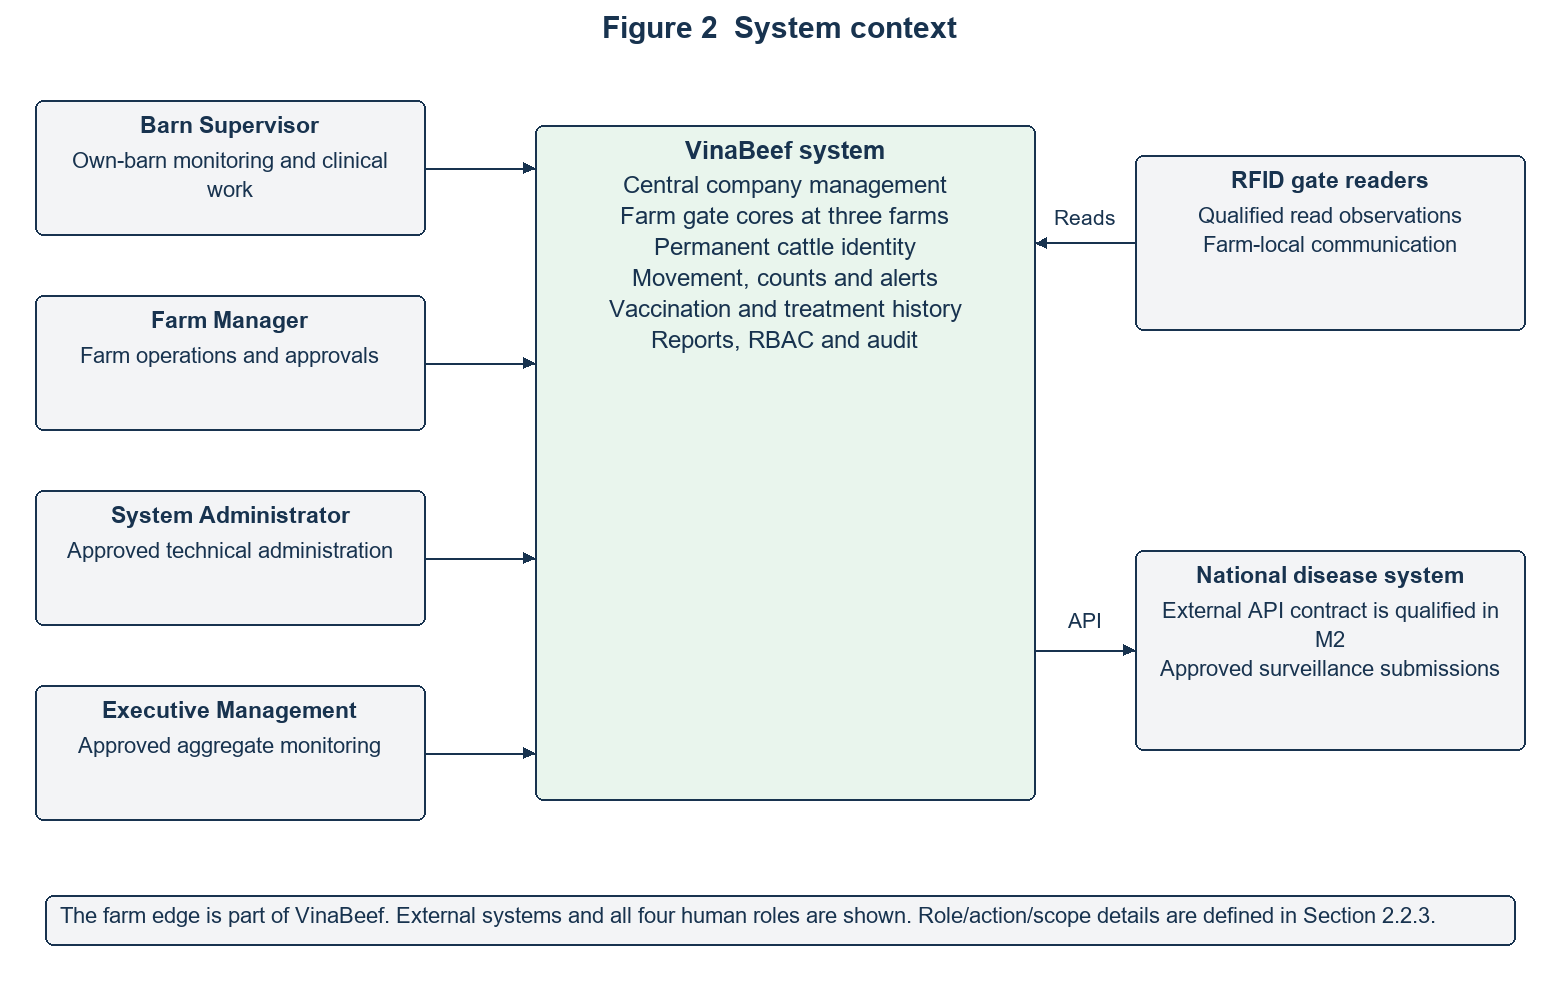
\includegraphics[width=\linewidth,height=0.42\textheight,keepaspectratio]{graphics/vinabeef/fig02-system-context.png}
\caption{System context with all four human roles}\label{fig:2}\end{figure}

\begin{figure}[htbp]\centering
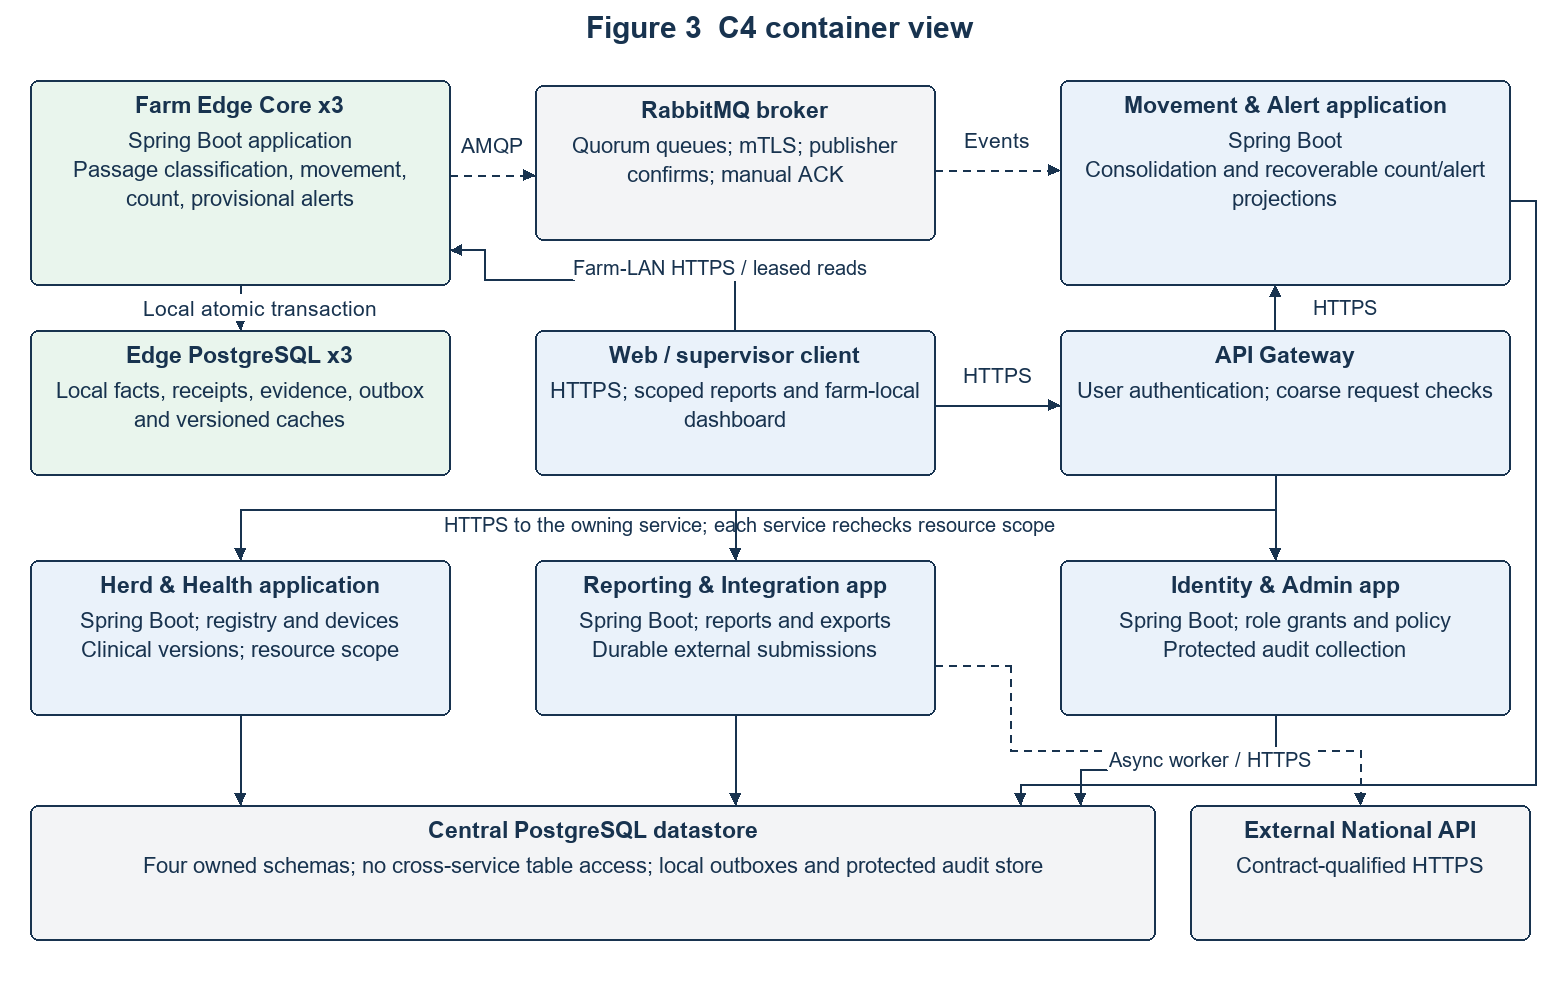
\includegraphics[width=\linewidth,height=0.42\textheight,keepaspectratio]{graphics/vinabeef/fig03-c4-containers.png}
\caption{C4 containers as applications and datastores}\label{fig:3}\end{figure}

\begin{figure}[htbp]\centering
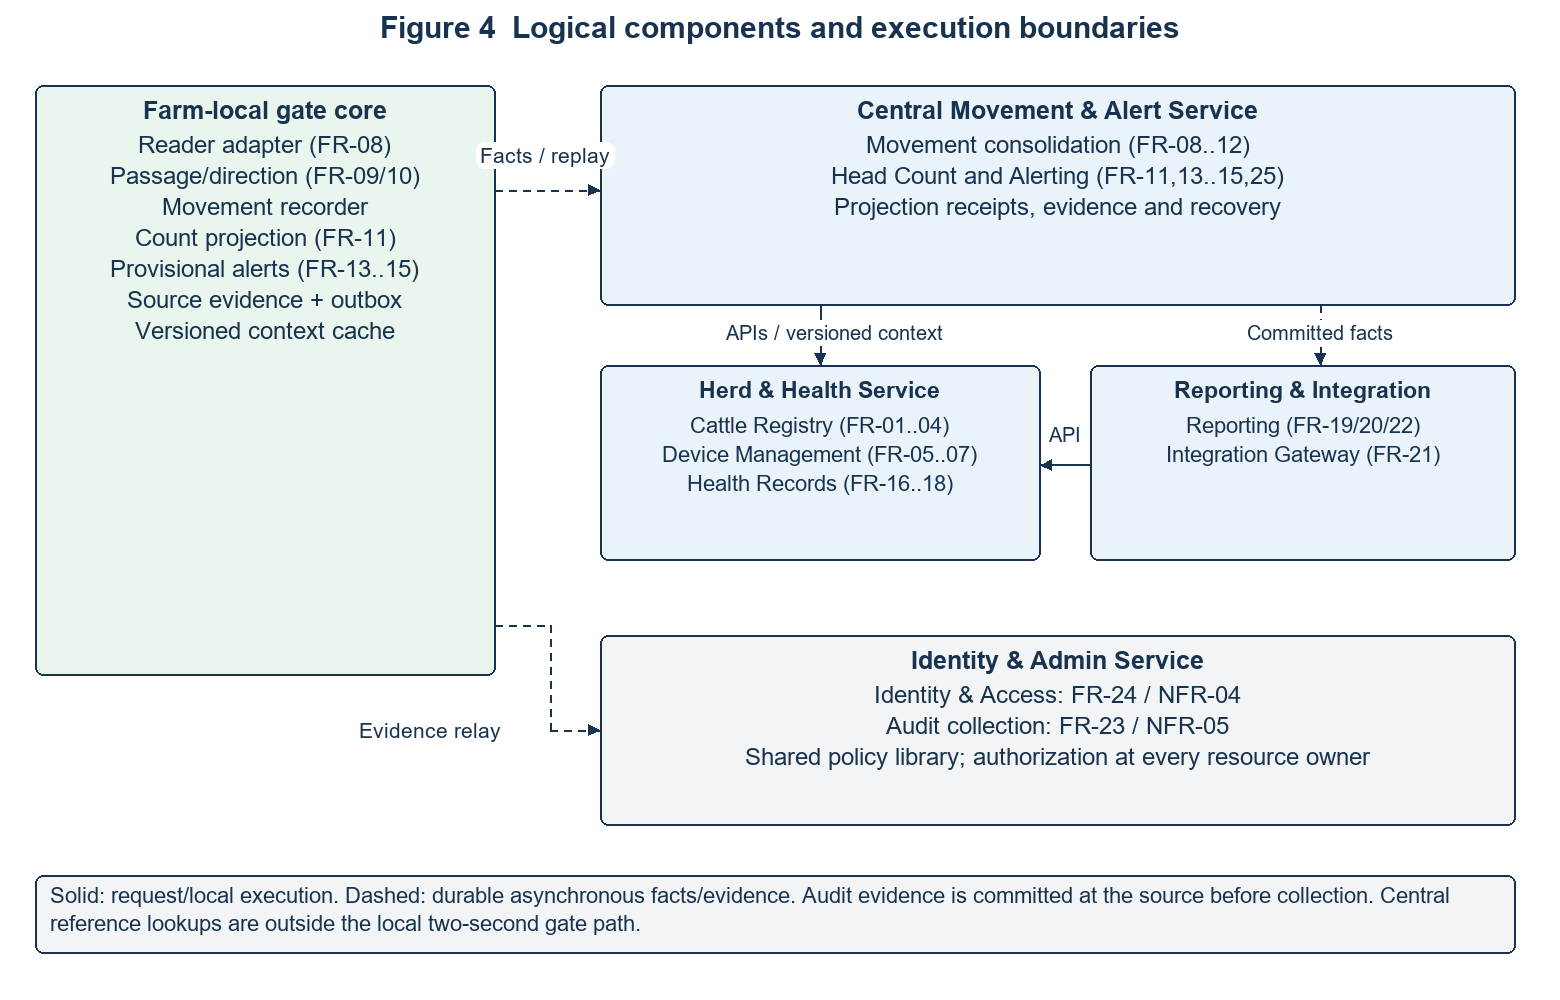
\includegraphics[width=\linewidth,height=0.42\textheight,keepaspectratio]{graphics/vinabeef/fig04-logical-components.png}
\caption{Logical components and farm/central execution boundaries}\label{fig:4}\end{figure}

\subsection{Physical Architecture}\label{sec:4.5}

\subsubsection{Step 1: Group components into deployable units}

Grouping follows criticality, data cohesion, rate of change and
location. The local gate core is placed at the farm; four coarse central
applications isolate domain work. Timing and resource behaviour of this
grouping are measured in M2.

{\small
\begin{longtable}[]{|>{\raggedright\arraybackslash}p{\dimexpr 0.3233\linewidth-2\tabcolsep\relax}|>{\raggedright\arraybackslash}p{\dimexpr 0.3233\linewidth-2\tabcolsep\relax}|>{\raggedright\arraybackslash}p{\dimexpr 0.3233\linewidth-2\tabcolsep\relax}|}
\hline
\textbf{Deployable unit} & \textbf{Components and data} & \textbf{Location / reason} \\ \hline
\endhead
Farm Edge Core & Reader adapter, passage/direction, local
movement/count, provisional alert rules, receipts/evidence/outbox,
caches & Three farm nodes; no central dependency for local outcome \\ \hline
Movement \& Alert & Central movement facts, count/alert projections,
projection receipts and outbox workers & Central; common movement domain
and recoverable projections \\ \hline
Herd \& Health & Cattle Registry, Health Records, Device Management &
Central; protected identity/custody/clinical ownership \\ \hline
Reporting \& Integration & Reports, export jobs, approved submission
intents/attempts & Central; isolate read-heavy and external work \\ \hline
Identity \& Admin & Identity, scoped grants, approved configuration,
protected Audit collection & Central; policy administration and evidence
collection \\ \hline
Web / supervisor clients & Presentation and scoped queries; farm-local
dashboard under lease & User devices; no authorization bypass \\ \hline
\end{longtable}
}

\subsubsection{Step 2: Define nodes and protections}

{\small
\begin{longtable}[]{|>{\raggedright\arraybackslash}p{\dimexpr 0.3233\linewidth-2\tabcolsep\relax}|>{\raggedright\arraybackslash}p{\dimexpr 0.3233\linewidth-2\tabcolsep\relax}|>{\raggedright\arraybackslash}p{\dimexpr 0.3233\linewidth-2\tabcolsep\relax}|}
\hline
\textbf{Node} & \textbf{Runtime and protection} & \textbf{Declared limitation} \\ \hline
\endhead
Farm x3 & Qualified readers; isolated LAN; small SSD/UPS edge server;
Docker Edge Core; local PostgreSQL & No destructive-storage zero-loss
guarantee; source evidence and history retained \\ \hline
Central & API gateway; four Spring Boot apps; three-node RabbitMQ quorum
cluster; PostgreSQL primary/synchronous standby; daily backup/WAL
archive & Service replicas do not remove shared DB/common infrastructure
failures; M2 qualifies resources \\ \hline
Clients & Browser and supervisor app; HTTPS; restricted farm-local
dashboard & New human logins and clinical/transfer/config writes remain
online-only \\ \hline
National system & External HTTPS API qualified during M2 & Receiver
semantics are outside VinaBeef control \\ \hline
\end{longtable}
}

Only the API gateway is publicly exposed for client traffic. Central
services/broker/stores remain private; farm edge links use assigned mTLS
machine identities. The gateway authenticates, while each owner checks
canonical resource permissions. Backup recovery and complete storage
loss require separately qualified RPO/RTO; the assignment no-loss
requirement is normal-operation preservation.

Farms reach the central site only through an IPsec site-to-site VPN.
Every farm-to-central connection is initiated by the edge: (1) AMQP
upload of committed facts, (2) HTTPS pull of versioned assignments and
devices, and (3) HTTPS refresh of configuration and policy leases, so
the design works behind farm NAT. An ops zone hosts the container
registry for signed edge images (staged rollout) and the monitoring and
log aggregation service. Each edge keeps its local history until the
central watermark confirms it, plus 90 days, before archiving. A failed
edge box is replaced from the registry image and local backup, and edge
recovery time is tested in M2. The baseline edge sizing is 4 vCPU, 8 GB
RAM and a 256 GB SSD.

\begin{figure}[htbp]\centering
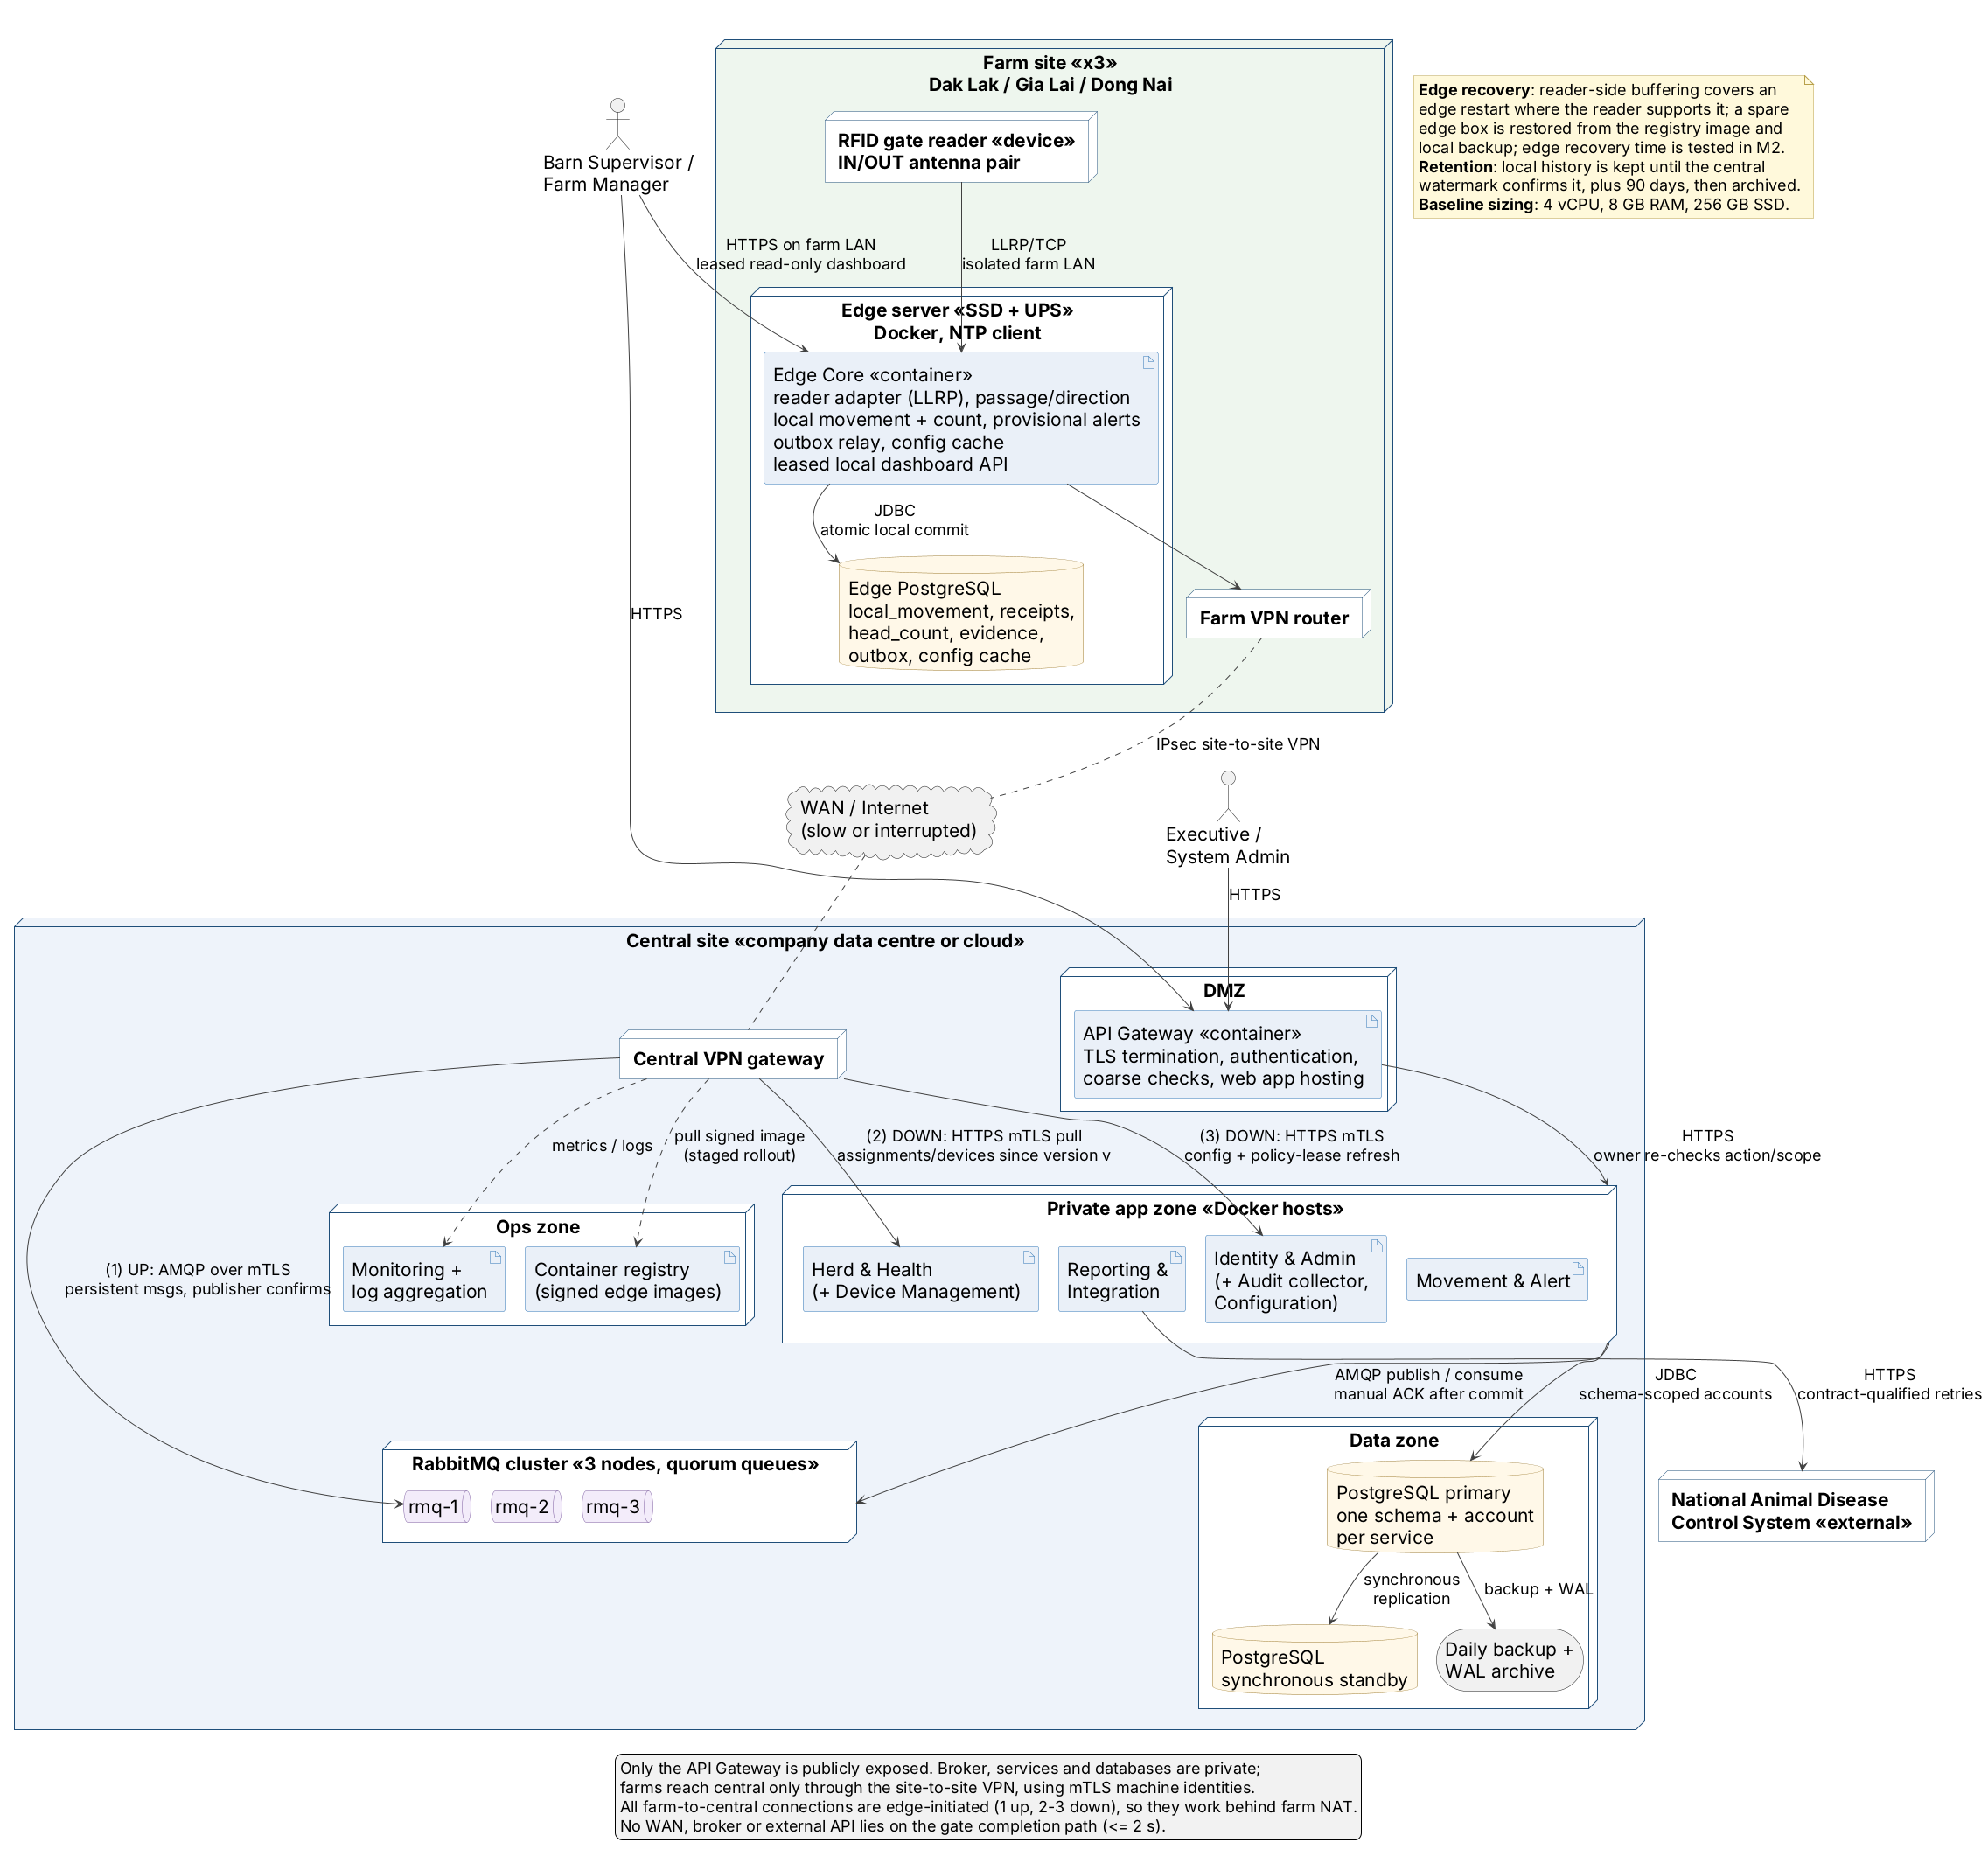
\includegraphics[width=\linewidth,height=0.8\textheight,keepaspectratio]{graphics/vinabeef/fig05-deployment.png}
\caption{Farm and central deployment with durable ownership}\label{fig:5}\end{figure}

\subsubsection{Step 3: Define communication and broker choice}

{\small
\begin{longtable}[]{|>{\raggedright\arraybackslash}p{\dimexpr 0.3233\linewidth-2\tabcolsep\relax}|>{\raggedright\arraybackslash}p{\dimexpr 0.3233\linewidth-2\tabcolsep\relax}|>{\raggedright\arraybackslash}p{\dimexpr 0.3233\linewidth-2\tabcolsep\relax}|}
\hline
\textbf{Link} & \textbf{Protocol} & \textbf{Completion semantics} \\ \hline
\endhead
Reader $\rightarrow$ Edge Core & Qualified LLRP/TCP farm-LAN adapter &
Source observations and application receipt semantics are established in
the reader contract \\ \hline
Edge $\rightarrow$ RabbitMQ $\rightarrow$ central & AMQP over
TLS/mTLS; persistent messages; quorum queues; publisher confirms; manual
consumer ACK & SENT\_TO\_BROKER proves broker receipt, not central
application completion \\ \hline
Client $\rightarrow$ owning service & Central HTTPS via gateway;
leased local HTTPS to farm Edge Core & Resource/approval checks at
service/query/export boundaries \\ \hline
Integration $\rightarrow$ external receiver & Qualified HTTPS API;
idempotency/status only if contract supports them & 202 remains pending;
unknown is retained; final evidence required \\ \hline
\end{longtable}
}

RabbitMQ is selected because this design needs durable work delivery,
per-consumer acknowledgements, redelivery and a stack the team can
configure and verify. The 200/1800 passage average is not a
raw-read/burst capacity bound. Kafka is a viable alternative for other
retention/replay or streaming needs; this project uses owned append-only
stores for history. Operational simplicity is a team assessment, not a
measured price comparison. M2 must qualify raw multiplicity, bursts,
concurrent farms, disk/CPU and recovery traffic.

\begin{figure}[htbp]\centering
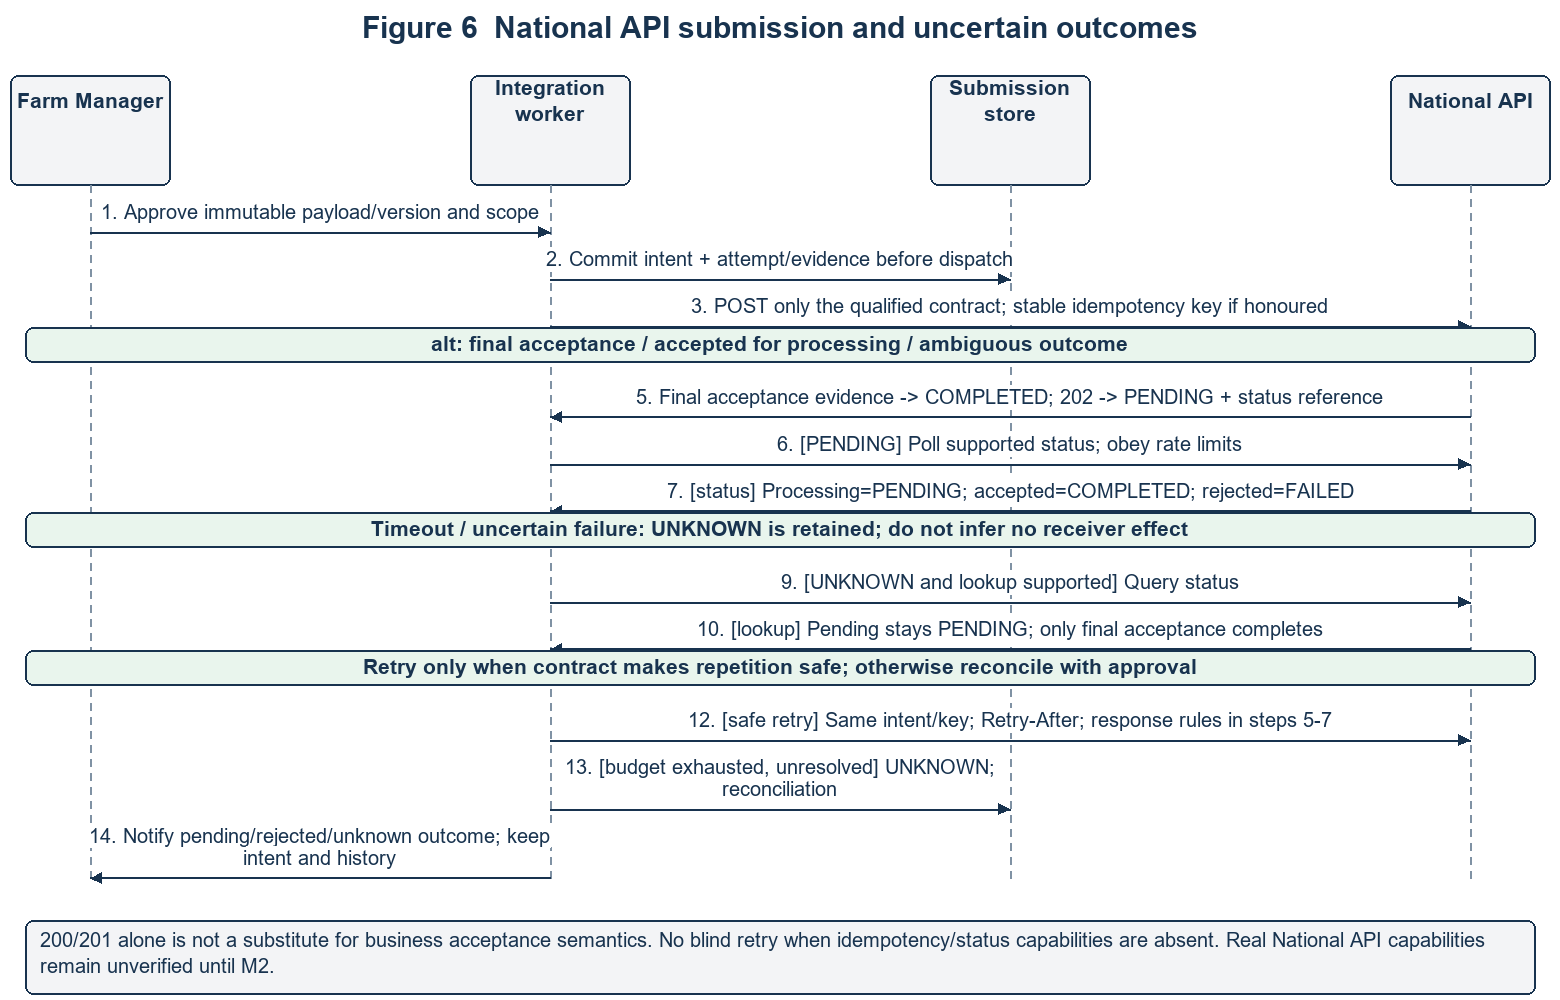
\includegraphics[width=\linewidth,height=0.42\textheight,keepaspectratio]{graphics/vinabeef/fig06-external-submission.png}
\caption{External submission with final acceptance and ambiguous-outcome handling}\label{fig:6}\end{figure}

\subsubsection{Step 4: Define owned data and domain invariants}

{\small
\begin{longtable}[]{|>{\raggedright\arraybackslash}p{\dimexpr 0.2904\linewidth-2\tabcolsep\relax}|>{\raggedright\arraybackslash}p{\dimexpr 0.2938\linewidth-2\tabcolsep\relax}|>{\raggedright\arraybackslash}p{\dimexpr 0.3858\linewidth-2\tabcolsep\relax}|}
\hline
\textbf{Store / owner} & \textbf{Data responsibilities} & \textbf{Write / recovery rule} \\ \hline
\endhead
Edge PostgreSQL / Edge Core & local\_movement; operation\_receipt;
local\_head\_count; source\_evidence; pending\_events outbox; versioned
assignment/config cache & Fact, effect, receipt and required evidence
commit atomically. SENT\_TO\_BROKER does not delete canonical local
history; duplicate/invalid dispositions remain durable. \\ \hline
Movement schema / Movement \& Alert & movement\_event;
processed\_event\_id; count/alert projections; projection receipts;
source\_evidence/outbox & Canonical facts append-only. Projection work
is durable and idempotent, with marker/effect/evidence committed per
projection owner. \\ \hline
Herd/Health schema & cattle permanentRFID; tag attachments/incidents;
devices; custody/transfer approvals; vaccination schedules and linked
clinical versions; receipts/evidence/outbox & Permanent RFID never
reassigned. Physical replacement preserves identity; different EPC is an
unapproved extension. Corrections append versions. \\ \hline
Reporting/Submission schema & report\_job; approved immutable
submission; payload hash/version; attempts; completion evidence &
Persist before dispatch; PENDING/UNKNOWN/COMPLETED/FAILED describe
business outcome. Unresolved exhaustion remains UNKNOWN. \\ \hline
Identity/Audit schema & human/machine principals; scoped RoleGrant;
policy version; protected audit\_record & No cross-service table access.
Canonical evidence is insert-only and references human or machine actor;
grants bind role and scope. \\ \hline
\end{longtable}
}

Stores may share the central PostgreSQL server, but accounts are limited
to owned schemas. Cross-owner access uses APIs/events and authorized
read models. Rebuild a projection only from a complete local history
plus its approved initial snapshot, or a verified central snapshot
merged with unsynchronized local facts. Compare equal source/event
watermarks first: ordinary eventual-consistency lag is not corruption.
Preserve original facts and evidence during reconciliation.

\begin{figure}[htbp]\centering
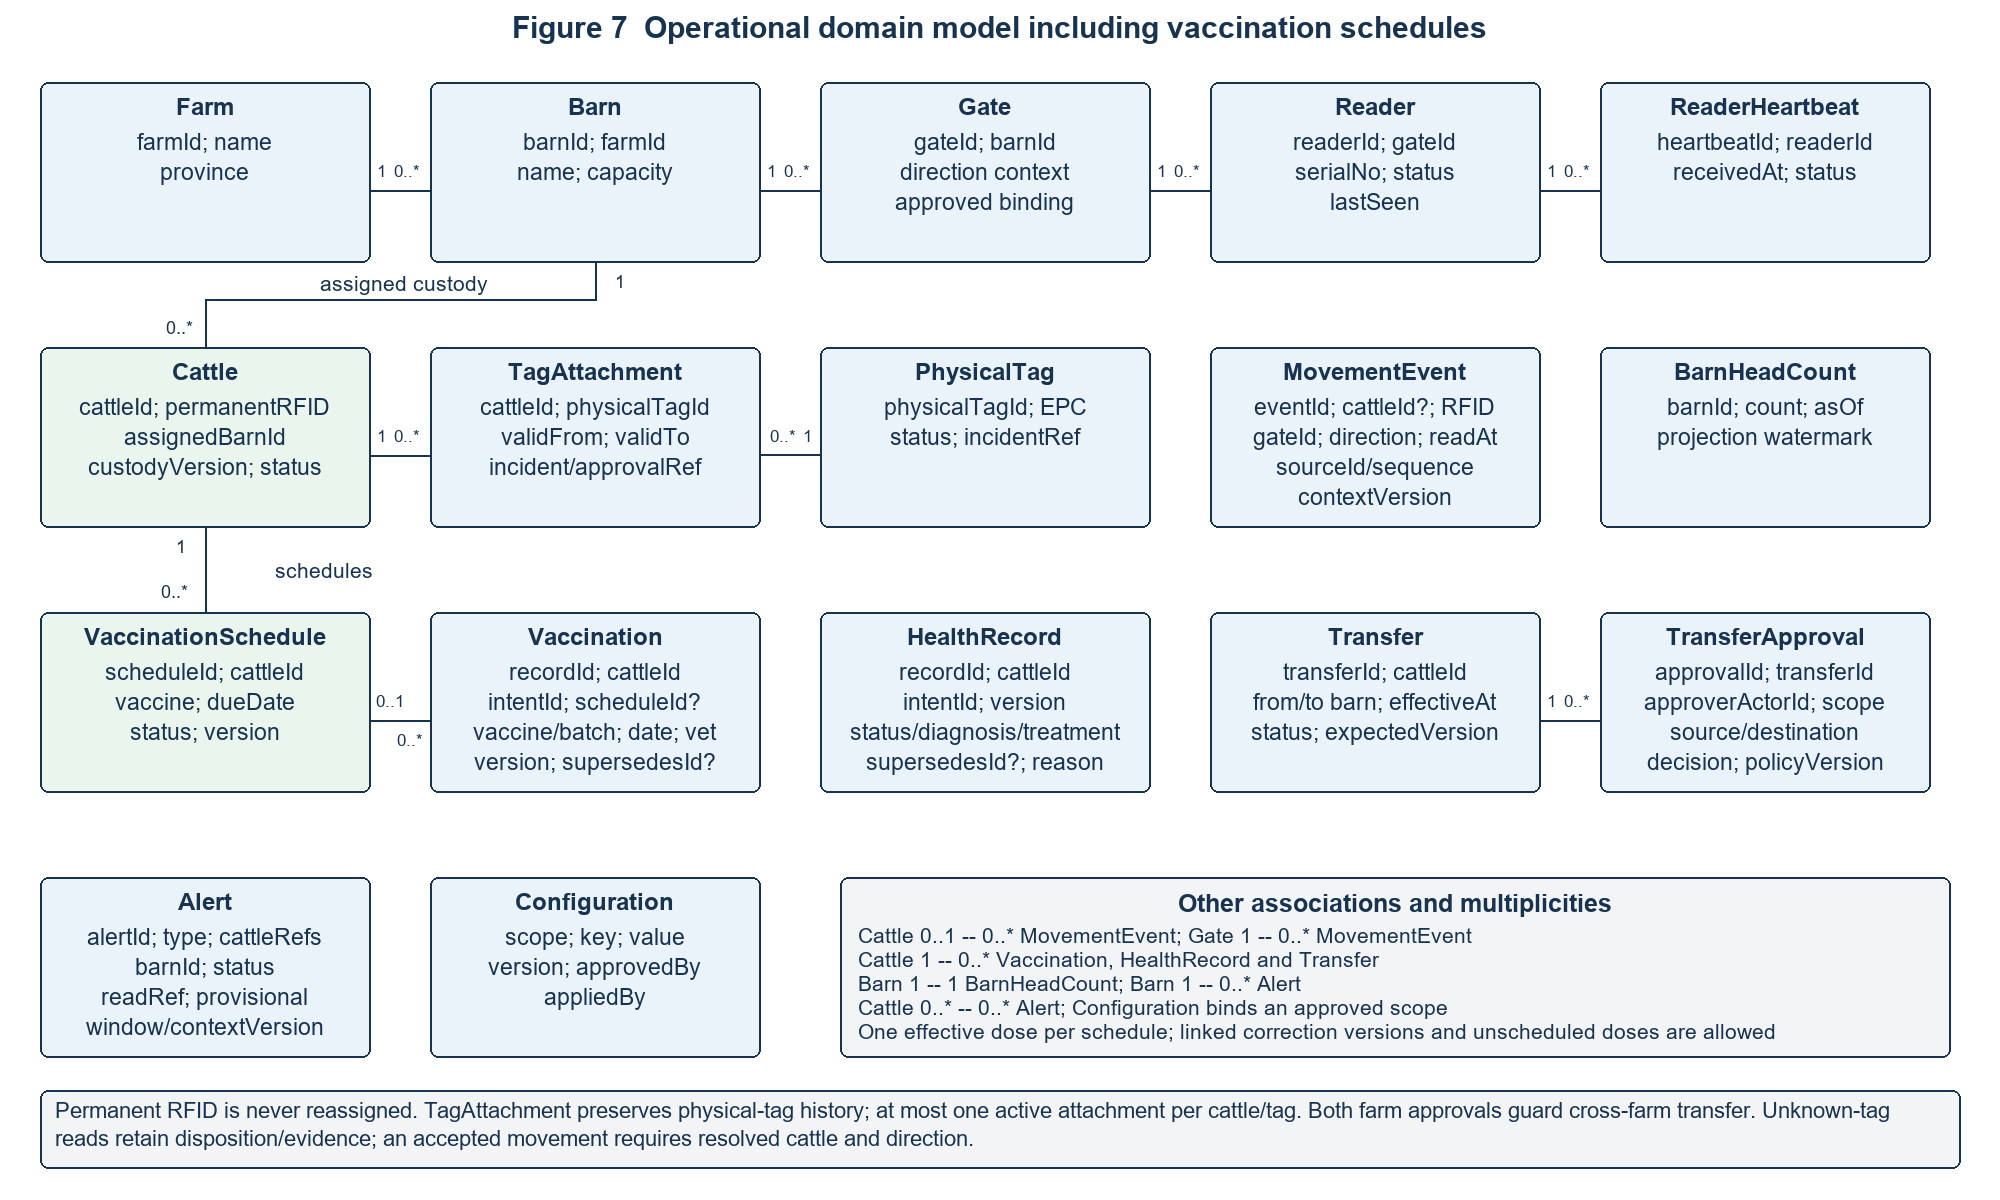
\includegraphics[width=\linewidth,height=0.42\textheight,keepaspectratio]{graphics/vinabeef/fig07-domain-entities.png}
\caption{Operational domain entities and immutable identity/custody constraints}\label{fig:7}\end{figure}

\begin{figure}[htbp]\centering
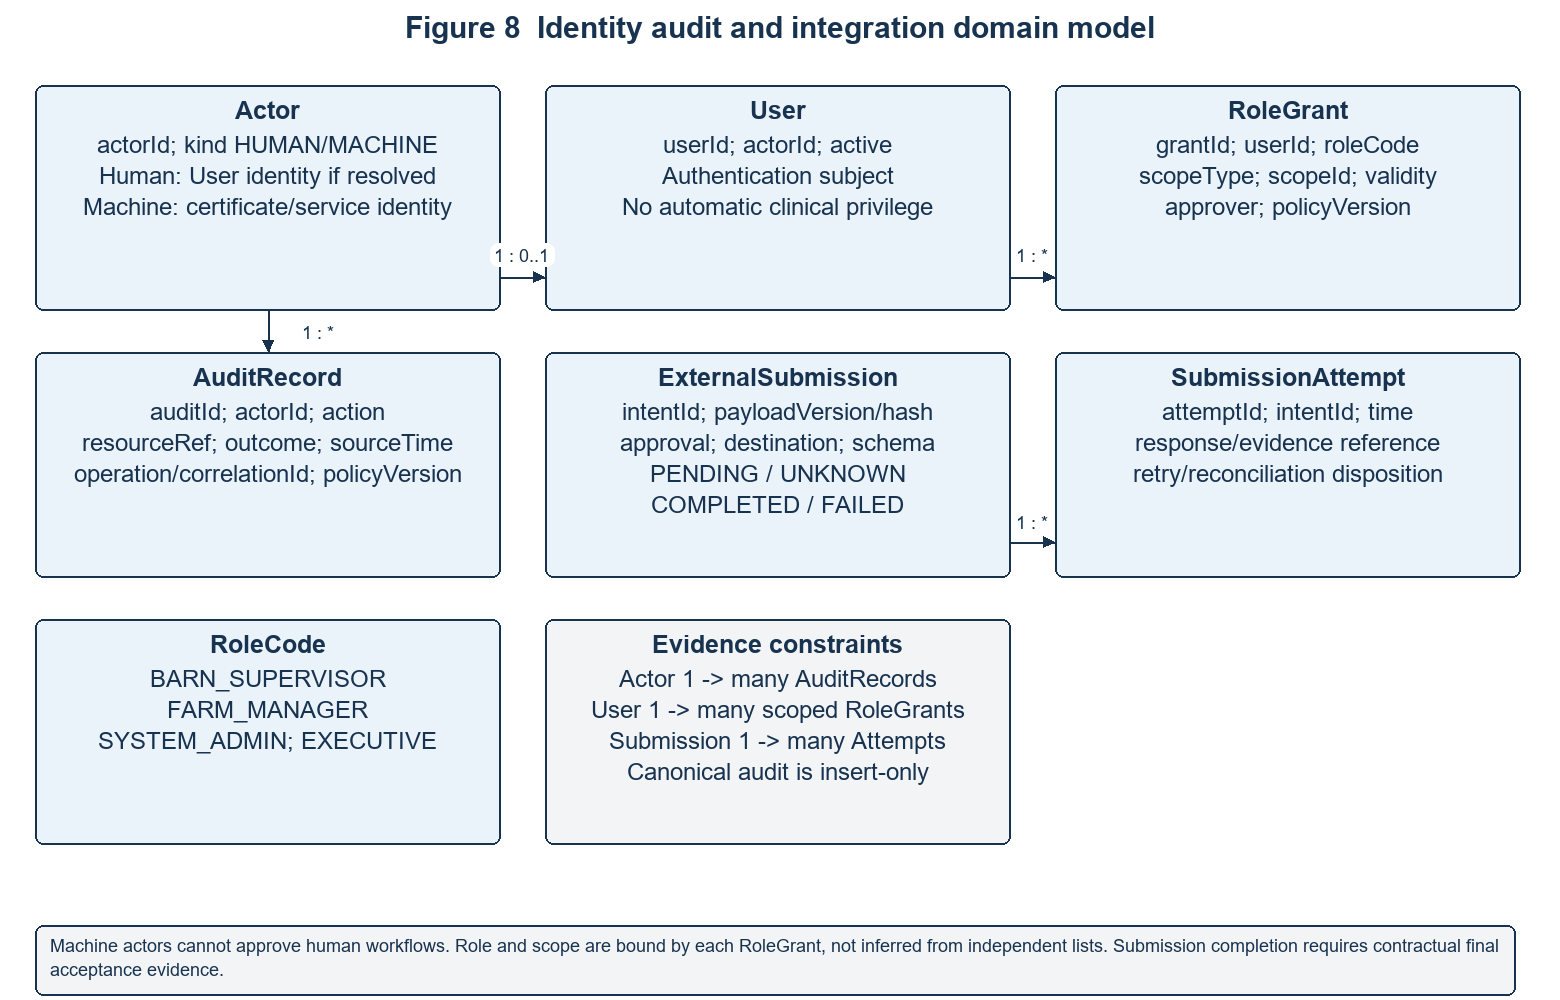
\includegraphics[width=\linewidth,height=0.42\textheight,keepaspectratio]{graphics/vinabeef/fig08-actors-grants.png}
\caption{Human/machine actors, scoped grants and external submission history}\label{fig:8}\end{figure}

\subsubsection{Step 5: Validate design walkthroughs and planned measurements}

Peak walkthrough: classify each qualified observation/passage and commit
the correct local disposition, movement/count effect and source evidence
within the SC-01 boundary. Raw-read bursts, source clock
uncertainty and resource limits are declared before M2 timing. Central
synchronization and the National API do not extend the local gate
critical path; placement alone is not a measured deadline guarantee.

Outage walkthrough: the gate core retains complete local facts,
receipts, count effects and evidence while context-dependent alerts are
provisional. Replay retains stable IDs and source sequence/event time;
late events cannot overwrite a newer state merely because they arrive
later. The 600-second recovery ends only when the outage cohort
is reconciled through central business facts, count/alert projections
and canonical evidence, while live local reads continue (SC-03).

Return-window walkthrough: match each OUT obligation with a later valid
IN and approved custody state; OUT/IN/OUT is missing again if its final
obligation remains open. BS acknowledgement and FM resolution are
distinct, audited actions. External walkthrough: final acceptance, 202,
rejection and timeout-after-effect have distinct outcomes; no
unsupported receiver capability is assumed.

\begin{figure}[htbp]\centering
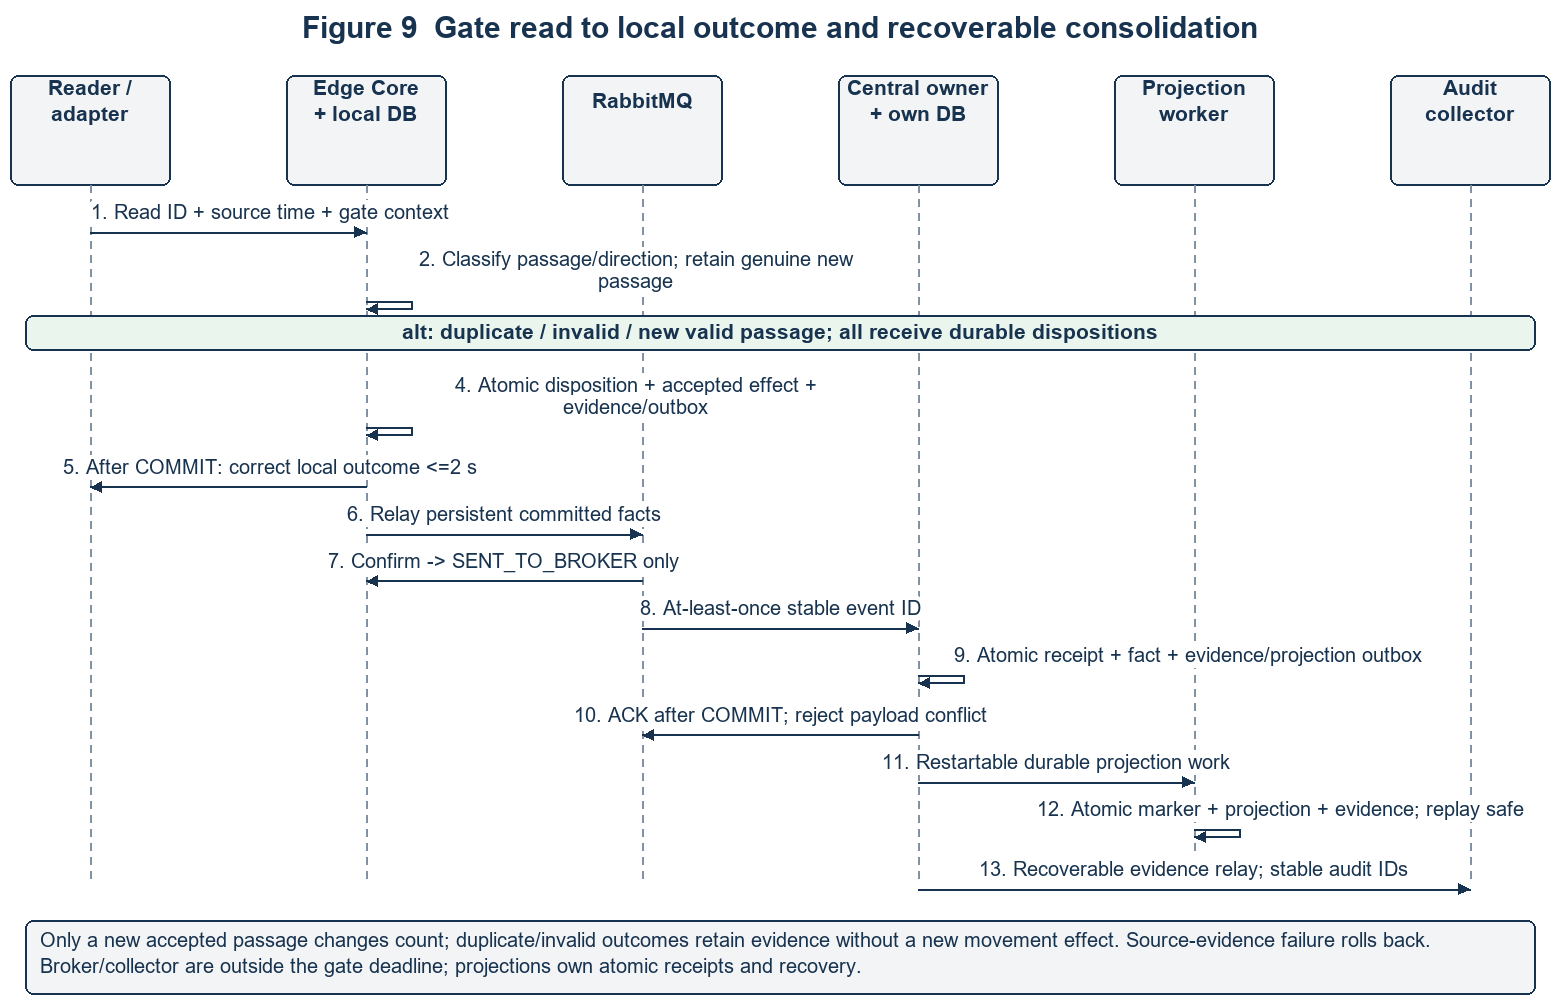
\includegraphics[width=\linewidth,height=0.42\textheight,keepaspectratio]{graphics/vinabeef/fig09-local-gate-outcome.png}
\caption{Durable local gate outcome and recoverable central projections}\label{fig:9}\end{figure}

\begin{figure}[htbp]\centering
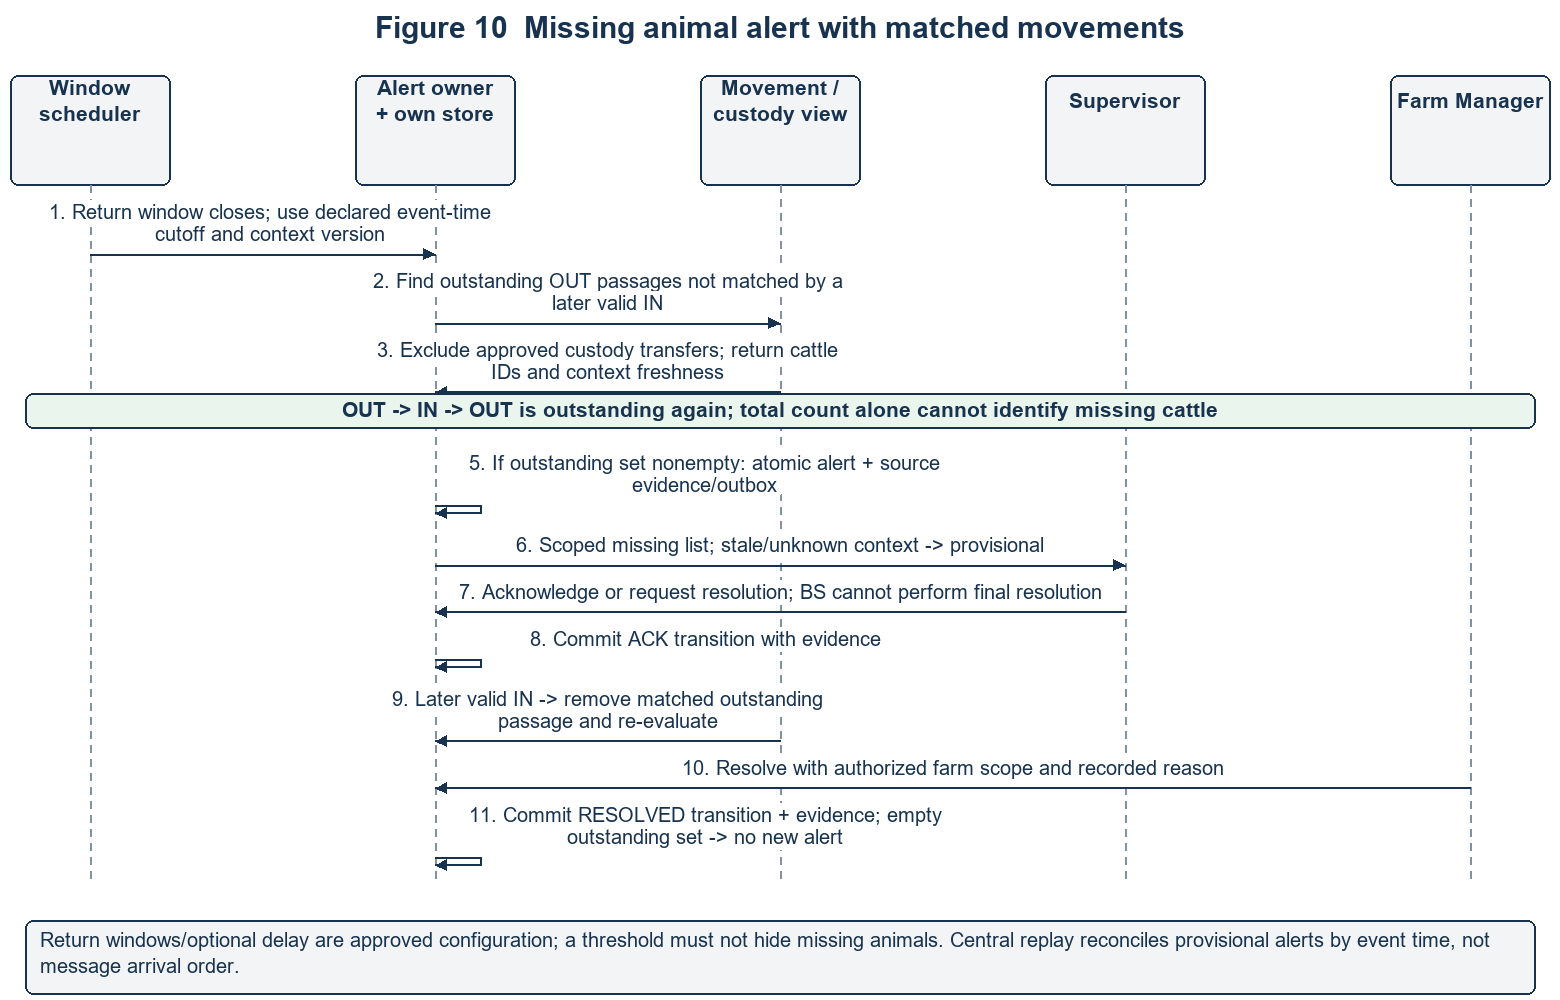
\includegraphics[width=\linewidth,height=0.42\textheight,keepaspectratio]{graphics/vinabeef/fig10-missing-detection.png}
\caption{Missing detection by outstanding movements and approved custody}\label{fig:10}\end{figure}

\begin{figure}[htbp]\centering
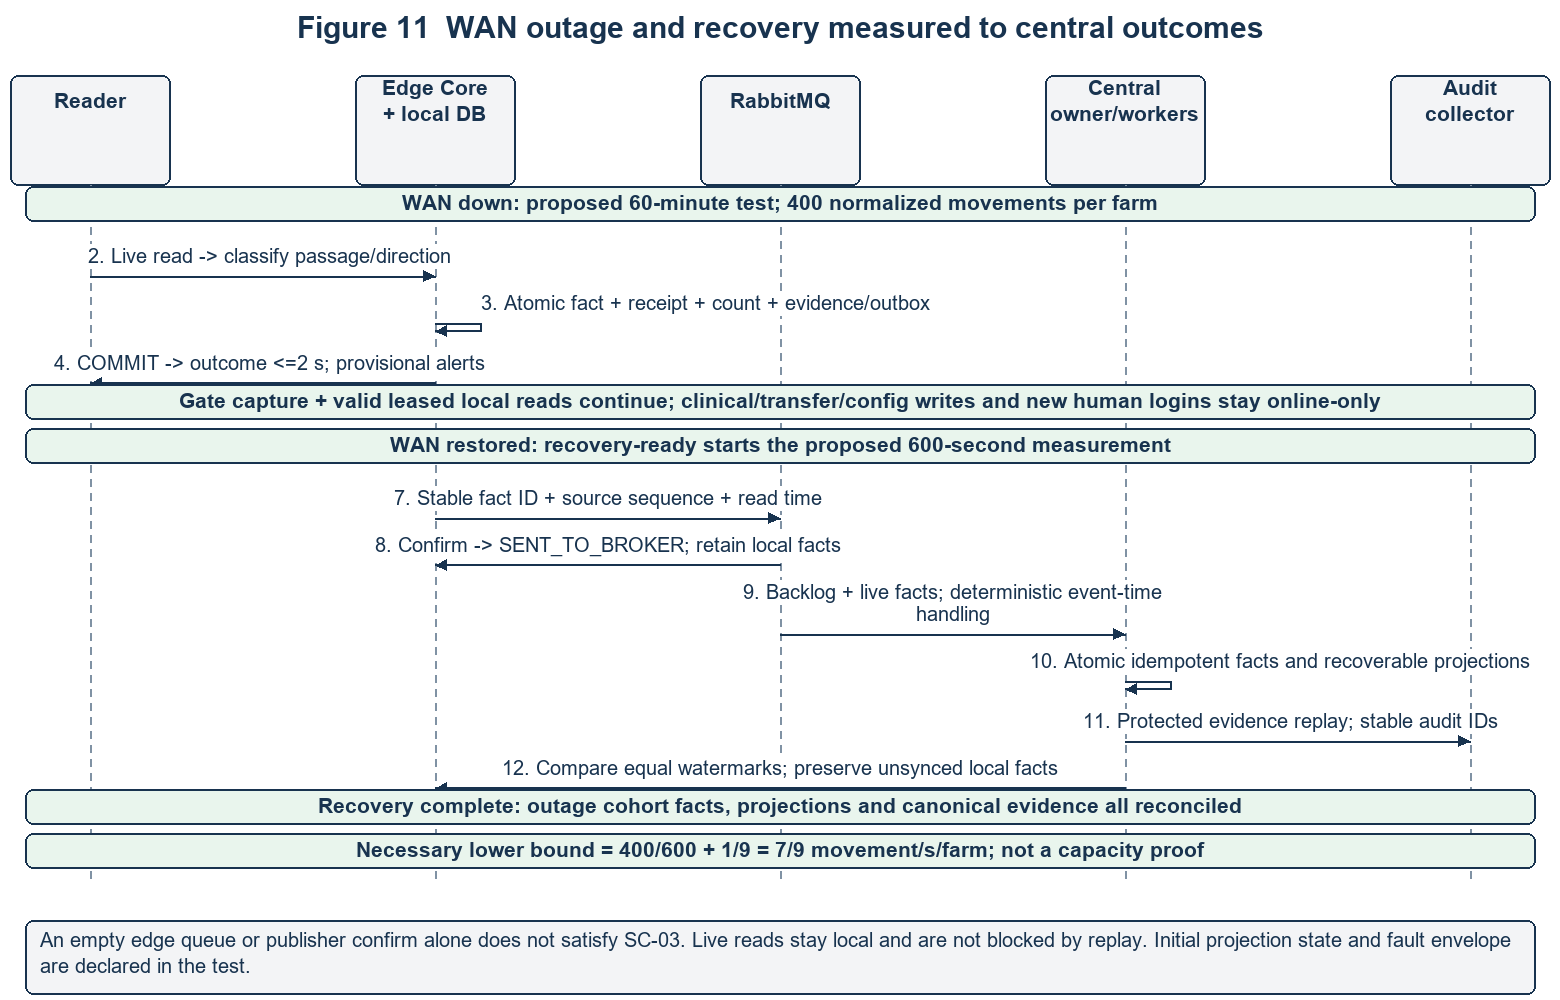
\includegraphics[width=\linewidth,height=0.42\textheight,keepaspectratio]{graphics/vinabeef/fig11-offline-capture.png}
\caption{Offline capture and recovery to completed central effects/evidence}\label{fig:11}\end{figure}
